\documentclass{beamer} %With pauses
% % \usepackage{fullpage}
\usepackage{framed}

% Figures
\usepackage{graphicx}
\usepackage{caption}
% \usepackage{subcaption}
\usepackage{wrapfig}
\usepackage{svg}

% Math packages, theorem definitions and numbering
\usepackage{amsmath}
\usepackage{amssymb}
\usepackage{amsthm}
\usepackage{mathrsfs} % Fancy scripted font
\usepackage{bm}  % Bold math
\usepackage{centernot}  % \centernot\implies looks better

% Misc packages
\usepackage[linesnumbered, ruled, vlined]{algorithm2e}
% \usepackage{algorithm2e} %{algorithm} environment
\usepackage{soul}  % \hl highlighting
\usepackage{color}
\usepackage{mathtools}  % For my \ceil function

% Theorems (with italics)
\theoremstyle{plain}  % Style definition removes italics
\newtheorem{theorem}{Theorem}
\newtheorem{corollary}{Corollary}
\newtheorem{proposition}{Proposition}
\newtheorem{lemma}{Lemma}

\theoremstyle{definition}
\newtheorem{remark}{Remark}
\newtheorem{definition}{Definition}
\newtheorem{example}{Example}
\newtheorem{assumption}{Assumption}

% keywords
\providecommand{\keywords}[1]{\textbf{\textit{Keywords---}} #1}

% General
\def\defeq{\overset{\Delta}{=}}  % Equal with triangle
\def\cl{\mathsf{cl\ }}  % Closure
\newcommand{\sgn}[1]{\mathsf{sgn}(#1)}  % sign function

% Calculus
\def\d{\mathsf{d}}  % Differential operator

% Functions
\def\ln{\mathsf{ln\ }}  % Natural logarithm
\DeclarePairedDelimiter{\ceil}{\lceil}{\rceil}  % Ceiling

% Probability
\def\H{\mathcal{H}}  % Hilbert space
\def\E{\mathbb{E}}  % Expectation
\def\Var{\text{Var}}  % Variance
\def\P{\mathbb{P}}  % Probability Measure
\def\F{\mathcal{F}}  % A sigma algebra
\def\sX{\mathcal{X}}  % Another sigma algebra
\def\KL{\mathbf{D}_{KL}}  % KL divergence
\def\bF{\mathbf{F}}  % Whole F-meas space
\def\GP{\mathcal{GP}}  % Gaussian process

% Standard sets
\def\Z{\mathbb{Z}}  % Set of integers
\def\R{\mathbb{R}}  % Set of real numbers
\def\C{\mathbb{C}}  % Set of complex numbers
\def\N{\mathbb{N}}  % Set of natural numbers
\def\ball{\mathbb{B}}  % Open ball
\def\clball{\overline{\ball}}  % Closed ball

% Linear algebra
\def\rk{\mathsf{rk }}  % The rank
\def\tr{\mathsf{tr }}  % The trace
\def\T{\mathsf{T}}  % Transpose notation
\def\c{\mathsf{c}}  % complement
\def\dg{\mathsf{dg }}   %  Diagonal vector of a matrix
\def\Dg{\mathsf{Dg }}   %  Diagonal matrix from a vector
\def\ind{\mathbf{1}}  % Ones vector or indicator
\def\matvec{\textbf{vec}}  % Vector operator
\def\<{\langle}  % < Inner product
\def\>{\rangle}  % > Inner product
\newcommand{\inner}[2]{\langle #1, #2 \rangle}  % Inner product
\newcommand{\innerT}[2]{#1^\T #2}  % Inner product for finite vectors

% Convex analysis
\def\conv{\mathsf{conv }}  % Convex hull
\def\prox{\mathsf{prox }}  % Proximity operator

% -----------------
% The given symbol or text (\text{mytext}) in a circle
% To be used always in math mode
\newcommand{\circlesign}[1]{ 
    \mathbin{
        \mathchoice
        {\buildcirclesign{\displaystyle}{#1}}
        {\buildcirclesign{\textstyle}{#1}}
        {\buildcirclesign{\scriptstyle}{#1}}
        {\buildcirclesign{\scriptscriptstyle}{#1}}
    } 
}

\newcommand\buildcirclesign[2]{%
    \begin{tikzpicture}[baseline=(X.base), inner sep=0, outer sep=0]
    \node[draw,circle] (X)  {\ensuremath{#1 #2}};
    \end{tikzpicture}%
}
% -----------------

%\documentclass[handout]{beamer} %Without pauses
\usepackage[backend=bibtex]{biblatex}
\usepackage{graphicx}
\usepackage{caption}
\usepackage{cancel}
\usepackage{centernot}
\usepackage[linesnumbered, ruled, vlined]{algorithm2e}
\usepackage{subcaption}

\usefonttheme[onlymath]{serif}

\setbeamertemplate{bibliography item}{}
\setbeamertemplate{bibliography entry title}{}
\setbeamertemplate{bibliography entry location}{}
\setbeamertemplate{bibliography entry note}{}

\addtobeamertemplate{navigation symbols}{}{%
    \usebeamerfont{footline}%
    \usebeamercolor[fg]{footline}%
    \hspace{1em}%
    \insertframenumber/\inserttotalframenumber
}

\bibliography{\string~/Documents/academics/global_academics/global_bib.bib}

\usepackage{wasysym}
\usepackage{tikz}

\usetheme{PaloAlto}

\newtheorem*{defn}{Definition}
\newtheorem*{proposition}{Proposition}

\def\E{\mathbb{E}}  % Expectation
\def\gc{\overset{\text{GC}}{\rightarrow}}  % Granger causality arrow
\def\ngc{\overset{\text{GC}}{\nrightarrow}}  % Negated Granger causality arrow
\def\pwgc{\overset{\text{PW}}{\rightarrow}}  % Pairwise Granger causality arrow
\def\npwgc{\overset{\text{PW}}{\nrightarrow}}  % Negated pairwise Granger causality arrow
\def\te{\overset{\mathcal{T}}{\rightarrow}}  % Transfer entropy arrow
\def\gcg{\mathcal{G}}  % Granger-causality graph
\def\gcge{\mathcal{E}}  % Graph edges
\def\VAR{\mathsf{VAR}}  % VAR(p) model
\def\B{\mathsf{B}}  % Filter B
\def\wtB{\widetilde{\B}}  % General filter B
\def\A{\mathsf{A}}  % Filter A
\def\H{\mathcal{H}}  % Hilbert space
\def\Ht{\mathsf{H}}  % Hermitian Transpose
\def\R{\mathbb{R}}  % Reals
\def\N{\mathbb{N}}  % Naturals
\def\T{\mathsf{T}}  % Transpose
\def\Z{\mathbb{Z}}  % Transpose
\def\cl{\mathsf{cl}}  % Closure
\def\ii{\mathsf{i}}  % Imaginary unit

\newcommand{\linE}[2]{\hat{\E}[#1\ |\ #2]}  % Linear projection
\newcommand{\linEerr}[2]{\xi[#1\ |\ #2]}  % Error of linear projection
\newcommand{\pa}[1]{pa(#1)}  % Parents of a node
\newcommand{\anc}[1]{\mathcal{A}(#1)}  % Ancestors of a node
\newcommand{\ancn}[2]{\mathcal{A}_{#1}(#2)}  % nth ancestors of a node
\newcommand{\gpn}[2]{gp_{#1}(#2)}  % nth generation grandparents
\newcommand{\wtalpha}[2]{\widetilde{\alpha}(#1, #2)}  % Some notation for lem:pwgc_anc
\newcommand{\dist}[2]{\mathsf{d}(#1, #2)}  % Distance between things
\newcommand{\gcgpath}[2]{#1 \rightarrow \cdots \rightarrow #2}  % A shorter path command

\title{Graph Topological Aspects of Granger Causal Network Learning}
\author{\texorpdfstring{Ryan J. Kinnear\newline\url{Ryan@Kinnear.ca}}{Ryan J. Kinnear}}% \author{Ryan J. Kinnear} \\
  % \small\href{mailto:ryan@kinnear.ca}{ryan@kinnear.ca} \\
  % \small\url{https://github.com/RJTK}\\
  % Under the Supervision of Ravi R. Mazumdar}

\institute[University of Waterloo] % (optional, but mostly needed)
{
  University of Waterloo\\
  Department of Electrical and Computer Engineering
}

\date{Fields-CQAM Student Workshop on Dynamical Systems and Related Fields, University of Waterloo, Oct 2019}

\AtBeginSection[]
{
  \begin{frame}<beamer>{Outline}
    \tableofcontents[currentsection,currentsubsection]
  \end{frame}
}

% Let's get started
\begin{document}

\begin{frame}
  \titlepage
\end{frame}

\begin{frame}{Outline}
  \tableofcontents
  % You might wish to add the option [pausesections]
\end{frame}

\section{Introduction}

% \begin{frame}{Causality}
%   \begin{itemize}
%     \item{Do billiard collisions cause motion?}\pause
%     \item{Does standing in the street cause cars to stop?}\pause
%     \item{Does smoking cause cancer?}\pause
%     \item{Does lowering interest rates cause lowering unemployment?}\pause
%     \item{Granger causality attemps to address the last question's category.}
%   \end{itemize}
% \end{frame}

% \begin{frame}{Causality in Time Series}
%   \begin{itemize}
%     \item{Consider $x_t, y_t \overset{\text{i.i.d.}}{\sim} \text{BER}(1/2)$}\pause
%     \item{If $z_t = x_{t - 1}$ then since cause preceeds effect, intuitively $x$ causes $z$}\pause
%     \item{$z'_t = x_{t - 1} \oplus y_{t - 1}$ is more ambiguous.}\pause
%     \item{Issue raised by: \fullcite{transfer_entropy_criticism}}\pause
%     \item{This difficulty is absent for \textit{linear} systems -- the domain of Granger causality}
%   \end{itemize}
% \end{frame}

\begin{frame}{Causality in Linear Time Series}
  \begin{itemize}
    \item{Granger causality formalizes ``cause proceeds effect'' for WSS processes}\pause
    \item{Interpretation as a ``Flow of Information'' or ``Flow of Energy'' is also reasonable}\pause
    \item{Given WSS processes, $x_1(t), \ldots, x_n(t)$, how can we understand causation $x_i \rightarrow x_j$?}\pause
    \item{\fullcite{granger1969investigating}}
  \end{itemize}
\end{frame}

\begin{frame}{Granger Causality}
  \begin{itemize}
    \item{Basic setup is an $n-$dimensional WSS process $x(t)$}\pause
    \item{$\mathsf{MA}(\infty)$ (Wold) representation $x(t) = \sum_{\tau = 0}^\infty A(\tau)v(t - \tau)$}\pause
    \item{$\VAR(\infty)$ representation $x(t) = \sum_{\tau = 1}^\infty B(\tau)x(t - \tau) + v(t)$}\pause
    \item{Require $\E[v(t)v(t - \tau)] = \delta_{\tau}\Sigma_v$, with $\Sigma_v$ Diagonal}\pause
  \end{itemize}

  \begin{defn}
    For the WSS series $x(t)$ we say that component $x_j$
    \textit{Granger-Causes} component $x_i$ (with respect to $x$)
    and write $x_j \gc x_i$ if

    \begin{equation*}
      \exists \tau > 0 \text{ s.t. } B_{ij}(\tau) \ne 0.
    \end{equation*}
  \end{defn}\pause

  % Need a VAR(2) definition of pairwise causality...
  % \begin{defn}
  %   We say that $x_j$ pairwise Granger-causes $x_i$ and write
  %   $x_j \pwgc x_i$ if $x_j$ Granger-causes $x_i$ with respect to
  %   $(x_i, x_j)$.
  % \end{defn}
\end{frame}

\begin{frame}{Simple Examples}
  \begin{equation*}
    x_i(t) = b_i x(t - 1) + v_i(t); i = 0, 1, 2
  \end{equation*}

  \begin{figure}
    \includegraphics[width=0.75\linewidth]{../figures/var1_example.pdf}
  \end{figure}
\end{frame}

\begin{frame}{Simple Examples}
  \begin{equation*}
    \begin{aligned}
      x_0(t) &= b_0 x_0(t - 1) + b_{0, 2} x_2(t - 150) + v_0(t)\\
      x_1(t) &= b_1 x_1(t - 1) + b_{1, 2} x_2(t - 150) + v_1(t)\\
      x_2(t) &= b_2 x_2(t - 1) + v_2(t)\\
    \end{aligned}
  \end{equation*}

  \centering
  \includegraphics[width=0.75\linewidth]{../figures/var2_example.pdf}
\end{frame}

\section{Causality Graphs}
\begin{frame}{Graph Terminology}
  \begin{itemize}
    \item{Graph $\gcg = (V, \gcge)$ with nodes (or vertices) $V$ and edges $\gcge$}\pause
    \item{Directed paths: $j \rightarrow a_0 \rightarrow \cdots \rightarrow a_r \rightarrow i$ for $(a_{k}, a_{k + 1}) \in \gcge$ distinct nodes}\pause
    \item{Cycles: paths with $i = j$}
    \item{Directed Acyclic Graph (DAG): A directed graph without any cycles}\pause
    \item{Parents: $j \in \pa{i}$ iff $(j, i) \in \gcge$}\pause
    \item{Ancestors: $j \in \anc{i}$ iff $j \rightarrow i$ path in $\gcge$}
  \end{itemize}
\end{frame}

\begin{frame}{Granger Causality Graph}
  A Granger causality graph is simply a graph $\gcg = ([n], \gcge)$
  with $(j, i) \in \gcge$ iff $j \gc i$.  $\VAR(1)$ models are
  particularly simple:

  \begin{columns}
    \begin{column}{0.25\textwidth}
      \includegraphics[width=1.5\linewidth]{../../figures/example1.pdf}
    \end{column}

    \begin{column}{0.75\textwidth}
      \begin{equation*}
        x(t) = \left[
          \begin{array}{cccc}
            0 & 0 & 0 & 0\\
            a & 0 & 0 & 0\\
            -a & 0 & 0 & 0\\
            0 & 1 & 1 & 0\\
          \end{array}\right]
        x(t - 1) + v(t)
      \end{equation*}
    \end{column}
  \end{columns}
\end{frame}

\begin{frame}{Granger Causality Graph}
  Structural results that tie in $\gcg$.  Recall:
  \begin{itemize}
    \item{$\mathsf{MA}(\infty)$ representation $x(t) = \sum_{\tau = 0}^\infty A(\tau)v(t - \tau)$}\pause
    \item{$\mathsf{VAR}(\infty)$ representation $x(t) = \sum_{\tau = 1}^\infty B(\tau)x(t - \tau) + v(t)$}\pause
  \end{itemize}

  \begin{proposition}
  $x_i(t)$ can be represented in terms of it's parents in $\gcg$:

  \begin{equation}
    \label{eqn:parent_expansion}
    x_i(t) = v_i(t) + \B_{ii}(z)x_i(t) + \sum_{k \in \pa{i}}\B_{ik}(z)x_k(t).
  \end{equation}\pause

  Or, through it's ancestors:

  \begin{equation}
    \label{eqn:ancestor_expansion}
    x_i(t) = \A_{ii}(z)v_i(t) + \sum_{\substack{k \in \anc{i} \\ k \ne i}}\A_{ik}(z)v_k(t).
  \end{equation}
    
  \end{proposition}
\end{frame}

% \begin{frame}{Application Examples}
%   Analysis of connectedness of financial institutions: 2002 - 2004

%   \begin{columns}
%     \begin{column}{0.75\linewidth}
%       \includegraphics[width=\linewidth]{../figures/finance_connections2002.png}
%     \end{column}
%   \end{columns}

%   \footfullcite{NBERw16223}
% \end{frame}

% \begin{frame}{Application Examples}
%   Analysis of connectedness of financial institutions: 2006 - 2008

%   \begin{columns}
%     \begin{column}{0.75\linewidth}
%       \includegraphics[width=\linewidth]{../figures/finance_connections2006.png}
%     \end{column}
%   \end{columns}

%   \footfullcite{NBERw16223}
% \end{frame}

% \begin{frame}{Application Examples}
%   Analysis of brain functional connectivity
  
%   \begin{columns}
%     \begin{column}{0.55\linewidth}
%       \includegraphics[width=\linewidth]{../figures/brain_photo.png}
%     \end{column}
%   \end{columns}

%   \footfullcite{anna_paper2008}
% \end{frame}

\begin{frame}{Application Example}
  Analysis of Gene regulatory networks
  
  \begin{columns}
    \begin{column}{0.5\linewidth}
      \includegraphics[width=\linewidth]{../../figures/ecoli_regulatory_network.pdf}
    \end{column}
  \end{columns}

  \footfullcite{discovering_graphical_Granger_causality_using_the_truncating_lasso_penalty}
\end{frame}

\section{Pairwise Causality and ``Causal Flow''}
\begin{frame}{Pairwise Granger Causality}
  \begin{itemize}
    \item{Suppose we observe only $x_i, x_j$ (components of a latent $x$)}\pause
    \item{Test \textit{pairwise} causality: $x_i \pwgc x_j$ (e.g. find
        the best $2-$dimensional model and check for zeros)}\pause
    \item{Statistical tests for the case $n = 2$ are simple and well established}\pause
    \item{Can we recover all of $\gcg$ by only testing pairwise relations?}\pause
    \item{Thresholding schemes suffer from confounding}\pause
    \item{\fullcite{tam2013gene_pwgc}}
  \end{itemize}
\end{frame}

\begin{frame}{Pairwise Causality}
  \begin{itemize}
    \item{Recall $j \pwgc i$ if $x_j$ Granger causes $x_i$ w.r.t $(x_i, x_j)$}\pause
  \end{itemize}
  
  \begin{columns}
    \begin{column}{0.5\textwidth}
      \begin{itemize}
        \item{Intuition suggests that $j \in \anc{i} \implies j \pwgc i$}\pause
      \end{itemize}

      \includegraphics[width=0.75\linewidth]{../../figures/example1.pdf}\pause
    \end{column}

    \begin{column}{0.5\textwidth}
      \begin{itemize}
        \item{At least $j \gc i \implies j \pwgc i$}\pause
      \end{itemize}
      \includegraphics[width=0.75\linewidth]{../../figures/example2.pdf}
    \end{column}
  \end{columns}
\end{frame}

\begin{frame}{Necessary Conditions for Pairwise Causality}
  \begin{itemize}
    \item{Interested in relationship between $x_j \gc x_i$ and $x_j \pwgc x_i$}\pause
  \end{itemize}

  \begin{proposition}
    Consider distinct nodes $i, j$ in a Granger causality graph $\gcg$.
    If

    \begin{enumerate}
      \item{$j \not\in \anc{i}$}\pause
      \item{$\anc{i}\cap\anc{j} = \emptyset$}\pause
    \end{enumerate}

    then $j \npwgc i$.
  \end{proposition}\pause

  \begin{itemize}
    \item{What about the simple graph $k \rightarrow i \rightarrow j$?}\pause
    \item{Surely $j \npwgc i$, even though $k \in \anc{i} \cap \anc{j}$?}
  \end{itemize}
\end{frame}

\begin{frame}{Necessary Conditions for Pairwise Causality}
  \begin{definition}[Confounder]
    A node $k$ is called a \textit{confounder} of nodes $i, j$ if
    $k \in \anc{i} \cap \anc{j}$ and there exists a path
    $\gcgpath{k}{i}$ not containing $j$, and a path $\gcgpath{k}{j}$
    not containing $i$.  A simple example is furnished by the ``fork''
    graph $i \leftarrow k \rightarrow j$.
  \end{definition}\pause

\begin{proposition}
  \label{prop:ancestor_properties}
  If in a Granger causality graph $\gcg$ where $j \pwgc i$ then
  $j \in \anc{i}$ or $\exists k \in \anc{i} \cap\anc{j}$ which is a
  confounder of $(i, j)$.
\end{proposition}
\end{frame}

\begin{frame}{Sufficient Conditions for Pairwise Causality}
  \begin{itemize}
    \item{Unfortunately, there is no general converse (e.g. recall $j \in \pa{i} \centernot\implies j \pwgc i$)}\pause
    \item{We seek special (graph-)\textit{topological} conditions when there is a converse}\pause
  \end{itemize}

  \begin{definition}[Strongly Causal]
    \label{def:strongly_causal}
    We will say that a Granger causality graph $\gcg$ is
    \textit{strongly causal} if there is at most one directed path between
    any two nodes.  Strongly Causal Graphs will be referred to as SCGs.
  \end{definition}
\end{frame}

\begin{frame}{Strongly Causal Graph Examples}
  \begin{columns}
    \begin{column}{0.5\linewidth}
      \small{Simple Example}
      \includegraphics[width=\linewidth]{../../figures/example_algorithm_step0.pdf}\pause
    \end{column}
    \begin{column}{0.5\linewidth}
      \small{Slightly larger example}
      \includegraphics[width=\linewidth]{../../figures/example_scg.pdf}
    \end{column}
  \end{columns}
\end{frame}

\begin{frame}{(Almost) Strongly Causal Graph Examples}
  \begin{columns}
    \begin{column}{0.5\linewidth}
      \small{E. Coli gene network \tiny{(\fullcite{discovering_graphical_Granger_causality_using_the_truncating_lasso_penalty})}}
      \includegraphics[width=\linewidth]{../../figures/ecoli_regulatory_network.pdf}\pause
    \end{column}
    \begin{column}{0.5\linewidth}
      \small{Saccharomyces cerevisiae gene network \tiny{(\fullcite{learning_genome_scale_regulatory_networks})}}
      \includegraphics[width=\linewidth]{../../figures/huge_gene_network.pdf}\pause
    \end{column}
  \end{columns}
\end{frame}

\begin{frame}{A Partial Converse}
  \begin{itemize}
    \item{In strongly causal (and acyclic) graphs, we have the appealing results:}
  \end{itemize}

  \begin{proposition}[Partial Sufficient Conditions]
    \label{prop:pwgc_anc}
    If $\gcg$ is a strongly causal DAG then $j \in \anc{i} \Rightarrow j \pwgc i$.
  \end{proposition}\pause

  \begin{corollary}
    \label{cor:gc_implies_pwgc}
    If $\gcg$ is a strongly causal DAG then $j \gc i \Rightarrow j \pwgc i$.
  \end{corollary}\pause

  \begin{itemize}
    \item{Unfortunately, effects of confounding more are nuanced}\pause
  \end{itemize}
\end{frame}

% \begin{frame}{Persistent Systems}
%   \begin{itemize}
%     \item{If $k \in \anc{i}\cap\anc{j}$ any of the following may occur:}\pause
%     \item{
%         $(i \npwgc j$, $j \npwgc i)$,
%         $(i \pwgc j$, $j \npwgc i)$,
%         $(i \npwgc j$, $j \pwgc i)$,
%         $(i \pwgc j$, $j \pwgc i)$}\pause
%     \item{Intuitively, $i$ may ``forget'' information from $k$ before the same information reaches $i$.}\pause
%   \end{itemize}

%   \begin{definition}[Persistent]
%     We will say that the process $x(t)$ with Granger causality graph
%     $\gcg$ is \textit{persistent} if every node has a self-loop,
%     i.e. $\B_{ii}(z) \ne 0$.
%   \end{definition}
% \end{frame}

% \begin{frame}{Persistent Systems}
%   Define $H_i(z)$ to be the filter s.t.:
  
%   \begin{equation*}
%     H_i(z)x_i(t) = \linE{x_i(t)}{\H_{t - 1}^{(i)}},
%   \end{equation*}\pause

%   And then with $\sigma_k^2 = \E v_k(t)^2$
%   \begin{equation*}
%     \label{eqn:T_filter}
%     T_{ij}(z) = \sum_{k \in \anc{i} \cap \anc{j}}\sigma_k^2\A_{ik}(z^{-1})(1 - H_i(z^{-1}))(1 - H_j(z))\A_{jk}(z)
%   \end{equation*}\pause

%   \begin{proposition}
%     \label{prop:persistence_converse}
%     Fix $i, j \in [n]$ and suppose $\exists k \in \anc{i} \cap \anc{j}$
%     which confounds $i, j$.  Then, if $T_{ij}(z)$ is not causal we have
%     $j \pwgc i$, and if $T_{ij}(z)$ is not anti-causal we have
%     $i \pwgc j$.  Moreover, if $T_{ij}(z)$ is two-sided, then $j \pwgc i \iff i \pwgc j$.
%   \end{proposition}
% \end{frame}

\section{Pairwise Testing Recovery Methods}
\begin{frame}{Pairwise Recovery}
  \begin{itemize}
    \item{Additional weak assumptions on $x$ are necessary to avoid pathological cancellation}\pause
    % \item{Persistant systems where $T_{ij}(z)$ is not two-sided are highly pathological}\pause
    \item{However, that the following requires an assumption on
        $T_{ij}(z)$ is an unfortunate blemish on the theory as it is
        not a topological requirement}\pause
  \end{itemize}

    \begin{theorem}[Pairwise Recovery]
      \label{thm:scg_recovery}
      If the Granger causality graph $\gcg$ for the process $x(t)$ is
      a strongly causal DAG and $T_{ij}(z)$ is two-sided for every
      $i, j$, then $\gcg$ can be recovered from pairwise causality
      tests alone.
    \end{theorem}

    \begin{itemize}
      \item{Proof is constructive in that I directly provide an algorithm to do so.}
    \end{itemize}
\end{frame}

\begin{frame}{Pairwise Recovery}
  \begin{algorithm}[H]
    \SetKwInOut{Input}{input}
    \SetKwInOut{Output}{output}
    \SetKwInOut{Initialize}{initialize}
    \DontPrintSemicolon

    \footnotesize
    % \BlankLine
    % \caption{Pairwise Granger Causality Algorithm}
    \label{alg:pwgr}
    % \TitleOfAlgo{Pairwise Graph Recovery}
    % \Input{Pairwise Granger causality relations between a persistent
    % process of dimension $n$ whose joint Granger causality
    % relations are known to form a strongly causal DAG $\gcg$.}
    % \Input{Pairwise Granger causality relations}
    % \Output{Edges $\gcge = \{(i, j) \in [n] \times [n]\ |\ i \gc j \}$ of
    %   the graph $\gcg$.}
    \Initialize{$S_0 = [n]$, $E_0 = \emptyset$, $k = 1$}\pause
    \BlankLine
    $W \leftarrow \{(i, j)\ |\ i \pwgc j, j \npwgc i\}$\\\pause
    $P_0 \leftarrow \{i \in S_0\ |\ \forall s \in S_0\ (s, i) \not\in W\}$\\\pause
    \While{$S_{k - 1} \ne \emptyset$}{
      $S_k \leftarrow S_{k - 1} \setminus P_{k - 1}$\\
      $P_k \leftarrow \{i \in S_k\ |\ \forall s \in S_k\ (s, i) \not\in W\}$\\\pause

      $D_{k0} \leftarrow \emptyset$\\\pause
      \For{$r = 1, \ldots, k$} 
      {
        $Q \leftarrow E_{k - 1} \cup \big(\bigcup_{\ell = 0}^{r - 1} D_{k\ell}\big)$\\\pause
        $D_{kr} \leftarrow \{(i, j) \in P_{k - r} \times P_k\ |\ (i, j) \in W,\ \text{no } i \rightarrow j \text{ path in } Q\}$\\\pause
      }
      $E_k \leftarrow E_{k - 1} \cup \big(\bigcup_{r = 1}^k D_{kr}\big)$\\\pause
      $k \leftarrow k + 1$\\\pause
    }
    \Return{$E_{k - 1}$}
  \end{algorithm}
\end{frame}

\begin{frame}{Pairwise Recovery}
  \begin{columns}
    \begin{column}{0.5\linewidth}
      \begin{figure}
        \includegraphics[width=\linewidth]{../../figures/example_algorithm.pdf}
      \end{figure}
    \end{column}

    \begin{column}{0.5\linewidth}
      \begin{figure}
        \includegraphics[width=\linewidth]{../../figures/example_algorithm_step0.pdf}
      \end{figure}
    \end{column}
  \end{columns}
\end{frame}

\begin{frame}{Pairwise Recovery}
  \begin{columns}
    \begin{column}{0.5\linewidth}
      \begin{figure}
        \includegraphics[width=\linewidth]{../../figures/example_algorithm0_step1.pdf}
      \end{figure}
    \end{column}

    \begin{column}{0.5\linewidth}
      \begin{figure}
        \includegraphics[width=\linewidth]{../../figures/example_algorithm_step0.pdf}
      \end{figure}
    \end{column}
  \end{columns}
\end{frame}

\begin{frame}{Pairwise Recovery}
  \begin{columns}
    \begin{column}{0.5\linewidth}
      \begin{figure}
        \includegraphics[width=\linewidth]{../../figures/example_algorithm0_step1.pdf}
      \end{figure}
    \end{column}

    \begin{column}{0.5\linewidth}
      \begin{figure}
        \includegraphics[width=\linewidth]{../../figures/example_algorithm_step1.pdf}
      \end{figure}
    \end{column}
  \end{columns}
\end{frame}


\begin{frame}{Pairwise Recovery}
  \begin{columns}
    \begin{column}{0.5\linewidth}
      \begin{figure}
        \includegraphics[width=\linewidth]{../../figures/example_algorithm0_step1.pdf}
      \end{figure}
    \end{column}

    \begin{column}{0.5\linewidth}
      \begin{figure}
        \includegraphics[width=\linewidth]{../../figures/example_algorithm_step2.pdf}
      \end{figure}
    \end{column}
  \end{columns}
\end{frame}

\begin{frame}{Pairwise Recovery}
  \begin{columns}
    \begin{column}{0.5\linewidth}
      \begin{figure}
        \includegraphics[width=\linewidth]{../../figures/example_algorithm0_step1.pdf}
      \end{figure}
    \end{column}

    \begin{column}{0.5\linewidth}
      \begin{figure}
        \includegraphics[width=\linewidth]{../../figures/example_algorithm_step3.pdf}
      \end{figure}
    \end{column}
  \end{columns}
\end{frame}

\begin{frame}{Pairwise Recovery}
  \begin{columns}
    \begin{column}{0.5\linewidth}
      \begin{figure}
        \includegraphics[width=\linewidth]{../../figures/example_algorithm0_step1.pdf}
      \end{figure}
    \end{column}

    \begin{column}{0.5\linewidth}
      \begin{figure}
        \includegraphics[width=\linewidth]{../../figures/example_algorithm_step4.pdf}
      \end{figure}
    \end{column}
  \end{columns}
\end{frame}

\section{Simulations}
\begin{frame}{Simulation}
  \begin{itemize}
    \item{Construct random graphs and compare PWGC against LASSO method}\pause
    \item{I obtained the best competing results with Zou's Adaptive
        LASSO -- but these methods are known to suffer somewhat from
        false positives}
    \item{\fullcite{adaptive_lasso_zou2006}}
  \end{itemize}
\end{frame}

\begin{frame}{Simulation}
  Representative Random Graph Topologies on $n = 50$ Nodes.  Parameter
  $q$ controls the density of edges.
  \begin{columns}
    \begin{column}{0.33\linewidth}
      \begin{figure}
        \caption{SCG}
        \includegraphics[width=\linewidth]{../../figures/example_scg.pdf}
      \end{figure}
    \end{column}\pause
    \begin{column}{0.33\linewidth}
      \begin{figure}
        \caption{DAG $(q = \frac{2}{n})$}
        \includegraphics[width=\linewidth]{../../figures/example_dag.pdf}
      \end{figure}
    \end{column}\pause
    \begin{column}{0.33\linewidth}
      \begin{figure}
        \caption{DAG $(q = \frac{4}{n})$}
        \includegraphics[width=\linewidth]{../../figures/example_dag_q.pdf}
      \end{figure}
    \end{column}
  \end{columns}
\end{frame}

\begin{frame}{Simulation}
  $\VAR(p)$ model with $n = 50, p = 15$ and randomized edge placements.  Left: SCG, Right: DAG ($q = 2/n$)
  \begin{columns}
    \begin{column}{0.5\linewidth}
      \includegraphics[width=0.9\linewidth]{../figures/new_lasso_comparison_scg_pmax15_simulation_mcc_only.png}
    \end{column}

    \begin{column}{0.5\linewidth}
      \includegraphics[width=0.9\linewidth]{../figures/new_lasso_comparison_dag_pmax15_simulation_mcc_only.png}
    \end{column}
  \end{columns}
\end{frame}

\begin{frame}{Simulation}
  \includegraphics[width=\linewidth]{../../figures/new_increasing_n_simulation.pdf}\pause
\end{frame}

\begin{frame}{Simulation}
  \includegraphics[width=\linewidth]{../../figures/new_mcc_comparison001.pdf}
\end{frame}

\section{Conclusion}
\begin{frame}{Conclusion}
  \begin{itemize}
    \item{The topology of $\gcg$, all else equal, may effect LASSO recovery}\pause
    \item{Granger causality suffers from some pathologies with ``causal flow''}\pause
    \item{$\gcg$ can be recovered from pairwise tests if it is strongly causal}\pause
    \item{Pairwise recovery algorithm performs surprisingly well, even if $\gcg$ is not strongly causal.}\pause
    \item{QUESTIONS?}
  \end{itemize}
\end{frame}

\end{document}
